% Adapted from: http://web.mit.edu/rsi/www/pdfs/beamer-tutorial.tex
\documentclass[pdf]{beamer}
\mode<presentation>{\usetheme{Warsaw} \useoutertheme{split}}
%\mode<handout>{\usecolortheme{seagull}}
%\usepackage{rsislidepacks}
\usepackage{amsfonts}
\usepackage{amsmath}
\usepackage{amssymb}
\usepackage{amsthm}
\usepackage{graphicx}
\usepackage{url}
\usepackage{pgfplots}
\usetikzlibrary{spy}
%

\usepackage{colortbl}
\usepackage{epstopdf}
\usenavigationsymbolstemplate{}
% title information
\title{Cloud and Big Data}
\subtitle{Big Data Overview}
\author{Gaurav Parashar \newline\url{gauravparashar24@gmail.com}
\newline{Lecture 1-3}}
\begin{document}

\AtBeginSection[]{
\begin{frame}{Table of Contents}
	\tableofcontents[currentsection]
\end{frame}
}

\begin{frame}
	\thispagestyle{empty}
	\titlepage
\end{frame}
\addtocounter{framenumber}{-1}

%%%%%%%%%%%%%%%%%%%%%%%%%%%%%%%%%%%%%%%%
\section{Objectives}
\begin{frame}{Objectives}
	\begin{itemize}
		\item Understand What is Big Data? \pause
		\item Analyse limitations of existing systems \pause
		\item Understand Hadoop and its features \pause
		\item Hadoop Ecosystem \pause
		\item Understand Hadoop 2.x core components \pause
		\item Perform read and write in Hadoop \pause
		\item Big Data and Cloud Lab Guidelines 
	\end{itemize}
\end{frame}


\section{Introduction}

%%%%%%%%%%%%%%%%%%%%%%%%
\subsection{What does "Big Data" Mean?}

\begin{frame}{What does "Big Data" Mean?}
	\begin{itemize}
		\pause
		\item Collecting large amounts of data
		\pause
		\begin{itemize}
			\item Computers, Databases, Video, Voice , tweets, comments, blogs, web pages, logs, calls, messages (Text + Whatsapp + ...) ,...
		\end{itemize}
	\end{itemize}
\pause
 What do we do with this data?	
\begin{itemize}
		\pause
		\item Early Fraud Detection, Credit Card Frauds, Tick~\cite{tic} Analytics 
		\pause
		\item Content personalisation, Recommendation System  
		\pause
		\item Insurance: Personalised Pricing
		\pause
		\item Customer Loyalty Data
		\pause
		\item Predicting Future
	\end{itemize}
\end{frame}
\subsection{Applications of Big Data}
\begin{frame}[fragile]{Applications of Big Data}
Examples: \\
Google Trends
	 \begin{figure}[ht]
	    \begin{center}
        		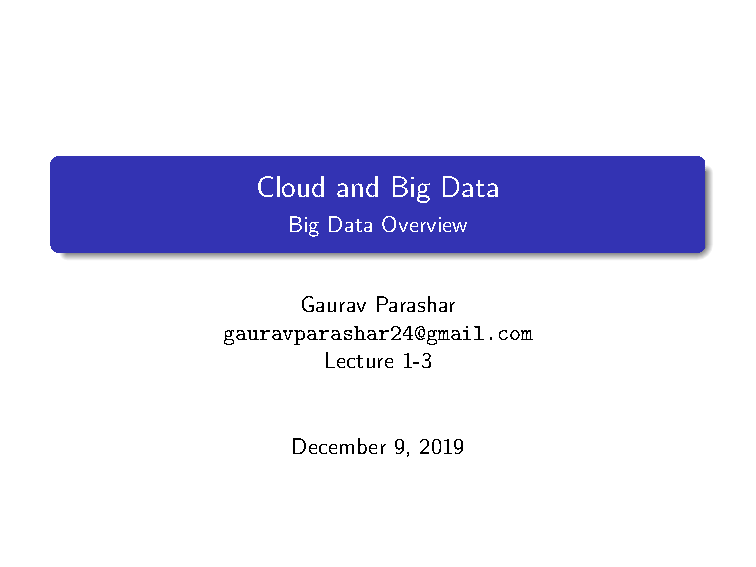
\includegraphics[height=2in]{1.png}
            ~\footnote{Google Trends for BJP and INC}
    \end{center}
    \end{figure}
\end{frame}
\begin{frame}[fragile]{Applications of Big Data}
Maps
	 \begin{figure}[ht]
	    \begin{center}
        		\includegraphics[height=2.2in]{2.png}
            ~\footnote{Display path, traffic, terrain, etd. time}
    \end{center}
    \end{figure}
\end{frame}

\begin{frame}[fragile]{Applications of Big Data}
Recommendation Systems
	 \begin{figure}[ht]
	    \begin{center}
        		\includegraphics[height=2.2in]{3.png}
            ~\footnote{Recommendation Engine}
    \end{center}
    \end{figure}
\end{frame}

\begin{frame}[fragile]{Applications of Big Data}
Twitter Trends
	 \begin{figure}[ht]
	    \begin{center}
        		\includegraphics[height=2in]{4.png}
            ~\footnote{Trending in Twitter}
    \end{center}
    \end{figure}
\end{frame}

\begin{frame}[fragile]{Applications of Big Data}
Big Data in Sports~\cite{GudmundssonH16}
	 \begin{figure}[ht]
	    \begin{center}
        		\includegraphics[height=2in]{6.png}
		\caption{Available receivers of pass by Red2}
            ~\footnote{Spatio-Temporal Analysis of Team Sports - {A} Survey}
    \end{center}
    \end{figure}
\end{frame}
\begin{frame}[fragile]{Applications of Big Data}
\begin{itemize}
    \item Weather Prediction
    \item Medical Diagnosis
    \item Smart Cities and Buildings
 \end{itemize}	
\end{frame}

\subsection[Generation of Big Data]{Generation of Big Data}
\begin{frame}[fragile]{Generation of Big Data}
	 \begin{figure}[ht]
	    \begin{center}
        		\includegraphics[height=2.9in]{5.jpg}
    \end{center}
    \end{figure}
\end{frame}

\section[5 Vs of Big Data]{5 Vs of Big Data}
%%%%%%%%%%%%%%%%%%%%%%%%%
%			Volume					%
%%%%%%%%%%%%%%%%%%%%%%%%%
\begin{frame}[fragile, label={vol}]{5 Vs of Big Data\cite{5vs}: Volume~\ref{iv1}}
\begin{tikzpicture}[spy using outlines ={magnification=2, circle, size=5cm, red, connect spies}]
\node (h1) at (0,0) {\includegraphics[height=2.9in]{7.png}};
\spy on (0.2,2.5)  in node at (6,1); 
\end{tikzpicture}
\end{frame}

\begin{frame}[fragile]{Scenario: Volume}
What is the staring limit of Big Data?
\begin{enumerate}[A]
\item $>$ 1 GB - $<$ 1TB \pause
\item  $>$ 1 TB - $<$ 1PB\pause
\item $>$ 1 PB - $<$ 1EB\pause
\item $>$ 1 EB - $<$ 1ZB\pause
\end{enumerate}
\uncover {Answer:}\\
\uncover {\small{Depends upon the organisation definition of Big Data. Relative term.}}

\end{frame}

\begin{frame}[fragile]{Scenario: Volume~\ref{iv1}}
 \begin{figure}[ht]
	    \begin{center}
        		\includegraphics[height=2.7in]{9.png}
    \end{center}
    \end{figure}
\end{frame}

%%%%%%%%%%%%%%%%%%%%%%%%%
%			Velocity					%
%%%%%%%%%%%%%%%%%%%%%%%%%
\begin{frame}[fragile, label={vel}]{5 Vs of Big Data: Velocity~\ref{iv1}}
\begin{tikzpicture}[spy using outlines ={magnification=1.7, circle, size=4.5cm, red, connect spies}]
\node (h1) at (0,0) {\includegraphics[height=2.9in]{7.png}};
\spy[thick, size=5cm] on (2.6,1.5)  in node at (6,-0.7); 
\end{tikzpicture}
\end{frame}


\begin{frame}[fragile]{5 Vs of Big Data: Velocity}
\begin{figure}[ht]
	    \begin{center}
        		\includegraphics[height=2.7in]{8.png}
    \end{center}
    \end{figure}
\end{frame}
%%%%%%%%%%%%%%%%%%%%%%%%%
%			Value					%
%%%%%%%%%%%%%%%%%%%%%%%%%
\begin{frame}[fragile, label={val}]{5 Vs of Big Data: Value~\ref{iv1}}
\begin{tikzpicture}[spy using outlines ={magnification=2, circle, size=4.5cm, red, connect spies}]
\node (h1) at (0,0) {\includegraphics[height=2.9in]{7.png}};
\spy[thick, size=5cm] on (2.5,-1.2)  in node at (6,1.7); 
\end{tikzpicture}
\end{frame}

%%%%%%%%%%%%%%%%%%%%%%%%%
%			Variability					%
%%%%%%%%%%%%%%%%%%%%%%%%%
\begin{frame}[fragile, label={var}]{5 Vs of Big Data: Variability~\ref{iv1}}
\begin{tikzpicture}[spy using outlines ={magnification=2, circle, size=5cm, red, connect spies}]
\node (h1) at (0,0) {\includegraphics[height=2.9in]{7.png}};
\spy[thick, size=5cm] on (0.2,-2.2)  in node at (6.1,1.7); 
\end{tikzpicture}
\end{frame}

%%%%%%%%%%%%%%%%%%%%%%%%%
%			Veracity					%
%%%%%%%%%%%%%%%%%%%%%%%%%
\begin{frame}[fragile, label={ver}]{5 Vs of Big Data: Veracity~\ref{iv1}}
\begin{tikzpicture}[spy using outlines ={magnification=2, circle, size=4.5cm, red, connect spies}]
\node (h1) at (0,0) {\includegraphics[height=2.9in]{7.png}};
\spy[thick, size=5.5cm] on (-2.1,-1.2)  in node at (5,1.7); 
\end{tikzpicture}
\end{frame}

%%%%%%%%%%%%%%%%%%%%%%%%%
%			Variety					%
%%%%%%%%%%%%%%%%%%%%%%%%%
\begin{frame}[fragile, label={vari}]{5 Vs of Big Data: Variety~\ref{iv1}}
\begin{tikzpicture}[spy using outlines ={magnification=2, circle, size=4.5cm, red, connect spies}]
\node (h1) at (0,0) {\includegraphics[height=2.9in]{7.png}};
\spy[thick, size=5cm] on (-2.3,1.2)  in node at (5,1.7); 
\end{tikzpicture}
\end{frame}

%%%%%%%%%%%%%%%%%%%%%%%%%
	%	Limitations of Existing Systems	%
%%%%%%%%%%%%%%%%%%%%%%%%%
\subsection{Limitations of Existing Systems}
\begin{frame}[fragile]{Limitations of Existing Systems}
\begin{enumerate}
	\item Cost of scaling \pause
	\item Vertical Scaling \pause
	\item Integration with legacy systems \pause
	\item Rapid Change in type of data \pause
	\item Lack of skills
\end{enumerate}
\end{frame}

%%%%%%%%%%%%%%%%%%%%%%%%%
	%	Industry Verticals	%
%%%%%%%%%%%%%%%%%%%%%%%%%
\section{Application of Big Data in Industry Verticals}
\subsection{Telecom}
\begin{frame}[allowframebreaks, label={iv1}]{Telecom}
A telco\cite{vtata} serving 8 million prepaid mobile subscribers
\begin{enumerate}
	\item Volume~\ref{vol}: \underline{amounting to 11 billion records annually}
	\item Velocity~\ref{vel}:  \underline{generates approximate 30 million CDR\cite{cdr}s daily}
	\item Value~\ref{val}: \underline{\hspace{3cm}}
	\item Variability~\ref{var}: \underline{\hspace{3cm}}
	\item Veracity~\ref{ver}:  \underline{\hspace{3cm}}
	\item Variety~\ref{vari}:  \underline{\hspace{3cm}}
\end{enumerate}
\end{frame}

\subsubsection{Call Detail Record}
\begin{frame}[fragile]{}
\begin{figure}[ht]
	    \begin{center}
        		\includegraphics[height=2.8in]{cdr.png}
    \end{center}
    \end{figure}
\end{frame}





%%%%%%%%%%%%%%%%%%%%%%%%
%References
%%%%%%%%%%%%%%%%%%%%%%%%%%%%%%%%%%%%%%%%
\section{References}
\bibliography{biblio} 
\bibliographystyle{ieeetr}
\end{document}
